
\subsection{Statistical Analysis}\label{sec-fitFramework}
After collecting the data and simulating the various samples, including the detector effects, reconstructing the physics objects, and applying the different cuts and the event categorisation, the last step in the analysis is to measure the signal yield normalised to the expected \gls{sm} yield (from theory, i.e., $\sigma \times BR$). The analysis aims to define a 95\% confidence level on the maximum signal enhancement factor $\mu$. This is done by maximising the binned-likelihood distribution in all of the analysis regions simultaneously as a function of the signal strength and statistical and systematic uncertainties. The full binned-likelihood function can be decomposed into three terms \cite{Mironova:2837159}: 
\begin{enumerate}
\item A Poisson probability term based on the expected and observed event yields in all bins of the considered distributions tracks the signal strength: $\mathcal{L} = \prod_{i\in \textrm{bins}} \textrm{Pois}(N_i \,|\, \mu s_i + b_i)$, where $N_i$, $s_i$, and $b_i$ are respectively the number of measured data events, the expected (simulated) signal yield, and the expected background yield in bin $i$. The signal strength parameter $\mu$ is the ratio of the measured $\sigma \times \textrm{BR}$ divided by the \gls{sm} expectation for the signal process.  
\item Systematics uncertainties enter the fit as Nuisance Parameters (NP) $\overrightarrow{\theta}$ which can modify the expected signal and background yields $s_i(\overrightarrow{\theta})$ and $b_i(\overrightarrow{\theta})$ in each bin. They are modelled as standardised Gaussian penalty terms: $\mathcal{L_{\textrm{NP}}} = \prod_{\theta \in \overrightarrow{\theta}} \frac{1}{\sqrt{2\pi}} e^{- \theta^2/2}$. After the fit, the values of the NPs can be moved upwards or downwards, and this deviation from 0 (from 1 for the normalisation factors) is called a \textit{pull}. The \textit{constraint} indicates the certainty on the value of the NP after the fit. NPs can have a prior, based on pre-existing knowledge or empirical estimates (e.g. auxiliary measurements, MC simulation model differences), or be left \textit{free-floating} (with a prefit value of 1), such as for the normalisation of the major backgrounds which is determined from data in control regions where these processes are enhanced. 
\item Uncertainties tracking the limited available statistics of the simulations are introduced as $\gamma_i$-parameters, with one such parameter per bin. They give the fit the flexibility to adjust the expected background yield in a particular bin as $b_i(\overrightarrow{\theta}) \rightarrow \gamma_i b_i(\overrightarrow{\theta})$. They are introduced as: $\mathcal{L_{\textrm{BkgStat}}}(\overrightarrow{\gamma}) = \prod_{i \in \textrm{bins}} \textrm{Gauss}(\beta_i | \gamma_i \beta_i, \sqrt{\gamma_i \beta_i})$, where $\beta_i = 1 / \sigma^2_\textrm{rel}$ and $\sigma_\textrm{rel}$ is the relative statistical uncertainty on the expected total background yield. 
\end{enumerate} 
The full likelihood function is then described as the product of these three contributions as 
\begin{equation}
\mathcal{L} = \prod_{i\in \textrm{bins}} \textrm{Pois}(N_i \,|\, \mu s_i(\overrightarrow{\theta}) + \gamma_i b_i(\overrightarrow{\theta})) \times  \prod_{\theta \in \overrightarrow{\theta}} \frac{1}{\sqrt{2\pi}} e^{- \theta^2/2} \times \prod_{i \in \textrm{bins}} \textrm{Gauss}(\beta_i | \gamma_i \beta_i, \sqrt{\gamma_i \beta_i}).
\end{equation}
For the signal, as previously described, a BDT score is used as a discriminant variable. Also called a \textit{Multivariate Analysis Discriminant} (MVA), one such BDT is trained per lepton channel, separately for $VH(H\rightarrow b\bar{b})$ and $VH(H\rightarrow c\bar{c})$. For the topCRs and the $\Delta R$ control regions, the invariant mass of the candidate pair  $m_{c\bar{c}}$ is used. \\

Systematic uncertainties, that act as priors and are constrained in the fit, on the simulated top background events (\textit{nominal samples}) are assessed by comparing the output of different setups of the simulator as well as using alternative simulators. Variations studied in these \textit{alternative samples} concern the matrix element generation (hard scattering), the renormalisation scale $\mu_R$ and factorisation scale $\mu_F$ for the ISR and FSR, the \textit{Parton Shower} (PS), the underlying event simulation, and multiple parton interactions \cite{Mironova:2837159}. Similar uncertainties are introduced for each of the other background processes. In addition, experimental uncertainties that affect all processes are introduced for the triggers, object reconstruction, flavour tagging, and the recorded data luminosity. They cover resolution effects, reconstruction efficiencies, and differences between data and simulations.\\

The different top components normalisations in 0L and 1L are determined from data in the profile likelihood fit by free-floating norm-factors (NF). A prior normalisation uncertainty is applied to account for potential differences between 0L and 1L. Acceptance ratios, in the number of jets and also in the extrapolation from the control region to the signal region, and shape uncertainties are also applied, after being derived for the top background in the 0L and 1L. When two top components are jointly floated, the dominated component is given an extra flavour ratio uncertainty to add flexibility to the fit. For example, when floating top($bl$) with top($bc$), the normalisation is mostly driven by top($bc$), the dominating component, and a ratio $bl$/$bc$ is added to let the $bl$ components adjust to differences between the two.  \\

The objective of this section is to study the impact of the modified top control regions on the combined 012L $VH(H\rightarrow c\bar{c})$ fit. The aim is to study for which top components the fit regions, and in particular the topCRs, provide enough information to determine their normalisation and constrain their shape from data. Furthermore, the data in the SRs should be sufficiently well described using the complete fit setup and the top background control regions should not significantly impact the behaviour (the NPs) of other backgrounds. While every bin of the analysis is used in the fit, bins with a large fraction of the signal (e.g., at high BDT score in the SRs) are not displayed as the analysis is still blinded. \\

Several iterations of the fit studies were performed to test the new topCRs proposed in this work and in particular which components can be constrained and which NPs can be correlated. The correctness of each fit is evaluated by verifying several diagnostics information, such as changes to the constraining of non-top-related NPs and to the predicted postfit yields. In the present report, three setups are presented to represent the evolution of the implementation of the topCR:
\begin{itemize}
\item Nominal: this is the first implementation to use all available topCRs (BT and BL) and the $VH(H\rightarrow b\bar{b})$ High $\Delta R$ CR with minimal changes to the other NPs. Other novelties introduced here are to free-float separately the top($bc$) and top($bl$) and to float the top($bb$) normalisation. The 2-jet and 3-jet regions share the same NFs and an additional 3-to-2-jet extrapolation uncertainty is implemented and applied in 2-jet. TopCR-SR extrapolation uncertainties are applied in the SRs except for top($lq$) where it is applied in the topCR. 
\item Baseline 2: uses only the topCR BT. Compared to the Nominal, the topCR BL is removed as it has a large $V$+jets background, especially in 0L, and impacts the NPs associated with this process, which is not the aim of the top control region. The top($bl$) is now floated jointly with top($bc$), as they are similar physics-wise since they both select a $b$-quark from the top-quark decay and a jet from the subsequent $W$ decay. An extra NP is introduced to model the $bl$ to $bc$ ratio. The main selection difference between the topCRs and the SRs is the tagging criteria. This difference should be covered by the flavour tagging uncertainties and the topCR-SR extrapolation uncertainties are therefore dropped. The flavour components represent different parts of the top components being selected as candidate jets. The difference induced in the 2-jet and 3-jet regions is not expected to be the same between the flavour components, hence the 3-to-2 jet extrapolation is decorrelated by flavour, separately for $t\bar{t}$ and $Wt$, marking the last modification with respect to the nominal setup.
\item Baseline 2 + nJetDec: is similar to Baseline 2 but now the topCR NFs are decorrelated on the number of jets. This is the preferred scenario if the data and CRs are powerful enough for the fit to converge since it maximally exploits the knowledge from the data and altogether avoids the need for 3-to-2 jet extrapolation uncertainties. These latter uncertainties can be very large because they cover different levels of mis-reconstructed or out-of-acceptance objects involved in the distinction of the top background into the 2-jet and 3-jet regions.
\end{itemize}

Figures \ref{fig:pullsTop} and \ref{fig:pullsFTAG} compare the pulls obtained by the different baselines considered. The top of Figure~\ref{fig:pullsTop} shows the floating normalisations of the top background. The [150, 250] GeV region is indicated by the \textit{BMin150} suffix and the region above 250 GeV by \textit{BMin250}, while the number of jets region is indicated by a suffix $J2$ or $J3$. All of the top components NFs are well constrained and the values obtained are consistent between the different $p_T^V$ regions and, for Baseline 2+nJetDec (in red), the number of jets regions. One small exception is the top($lq$) in Baseline 2+nJetDec. This component is however less relevant to the analysis and the top($lq$) can simply be kept inclusive in the number of jets in the final setup. Thanks to the inclusion of the CRHigh from $VH(H\rightarrow b\bar{b})$, even the top($bb$) component is well constrained in $VH(H\rightarrow c\bar{c})$. When removing the topCR BL, a small difference is induced in the NF for the V+jets background (not shown in the Figure). For example, the postfit yield of the W+jets background in the 1L [150, 250] GeV TT SR changes by 0.69\% between the Nominal and Baseline 2 + nJetDec (from 461000 to 457800 expected events). \\

\begin{figure}[h!]
%\hspace{-4.0cm}
\centering
\begin{subfigure}[b]{0.49\textwidth}
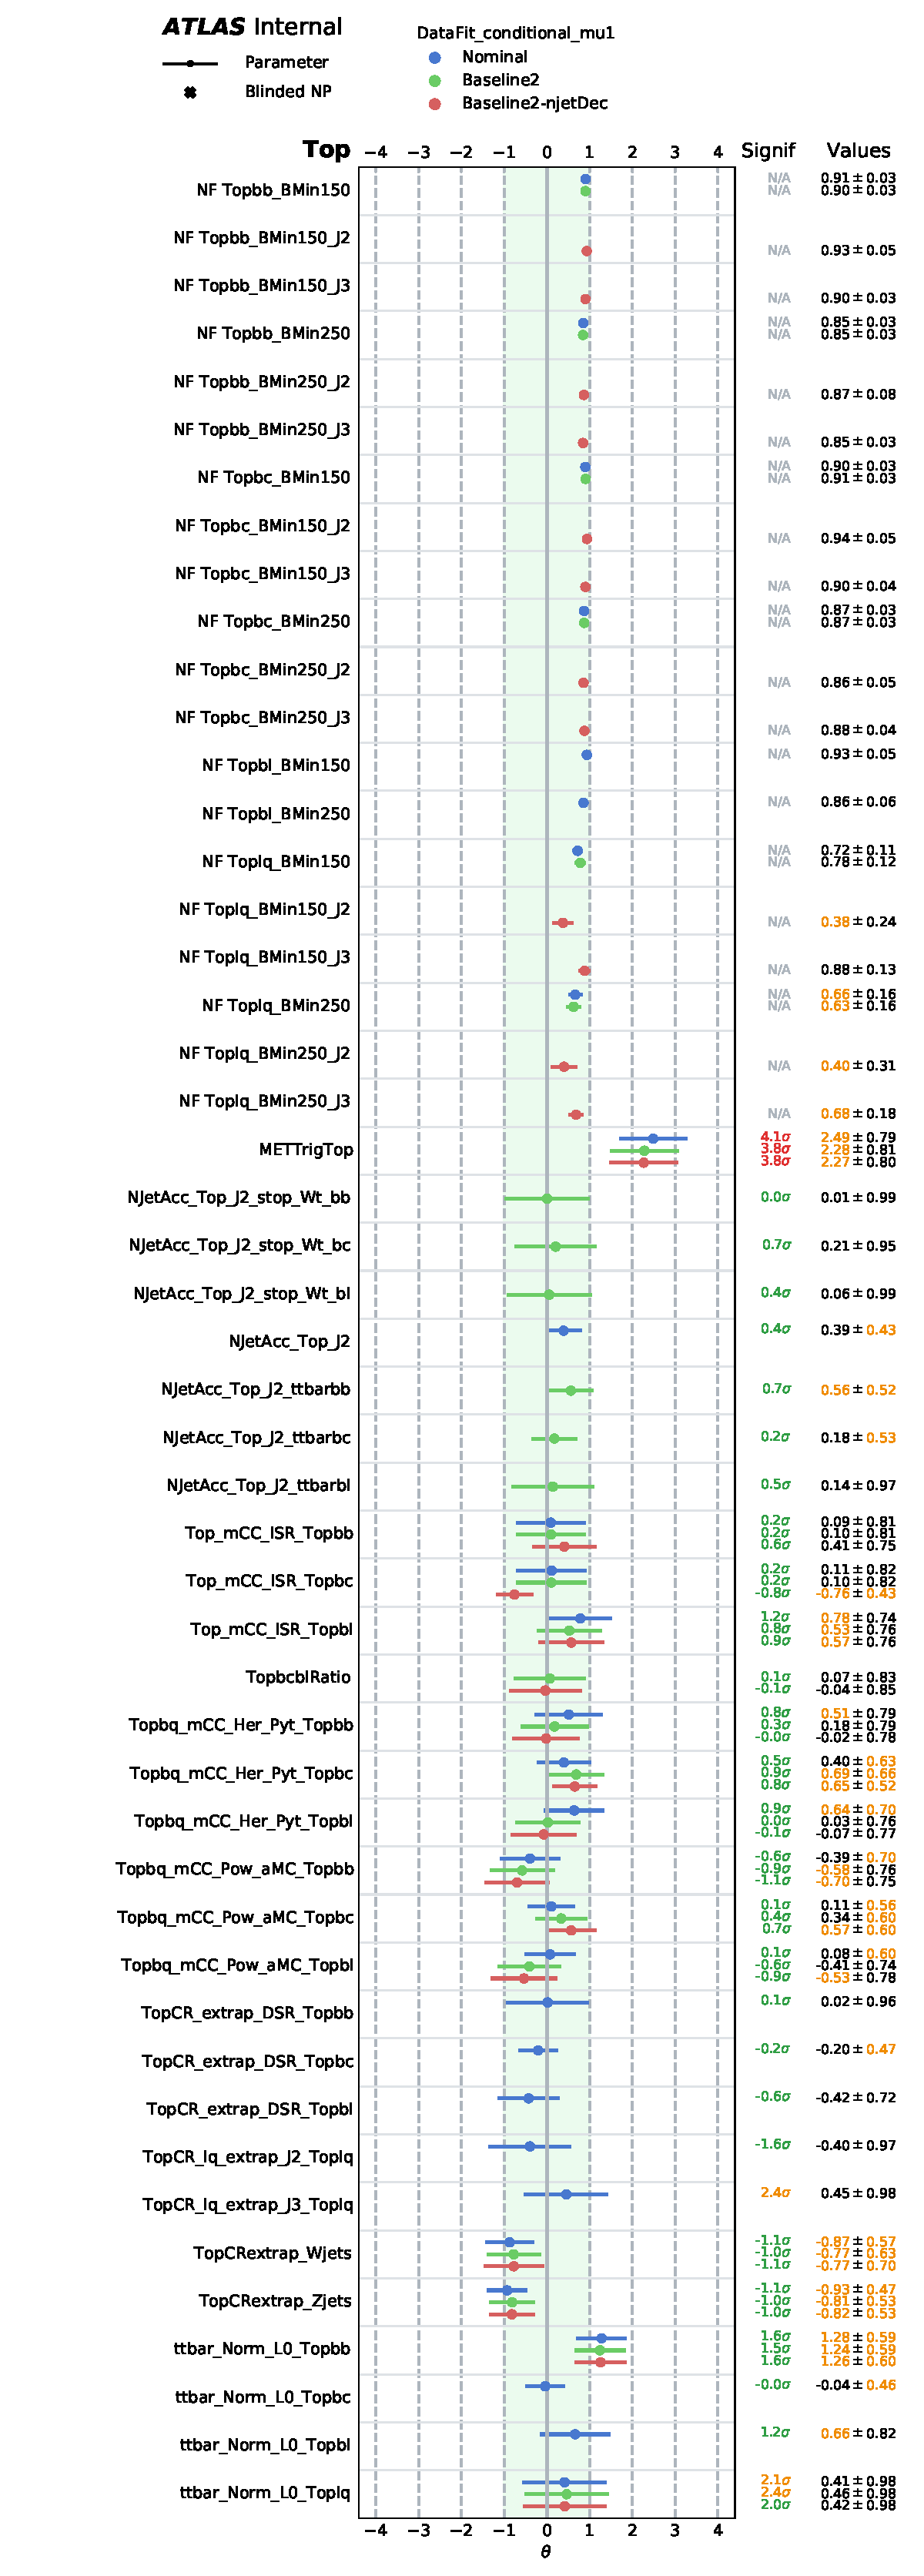
\includegraphics[scale=0.43]{Images/VH/clean_pull/NP_Top.pdf}
\caption{Top pulls.} 
\label{fig:pullsTop}
\end{subfigure}
 %
 \hfill
 %
\begin{subfigure}[b]{0.49\textwidth}
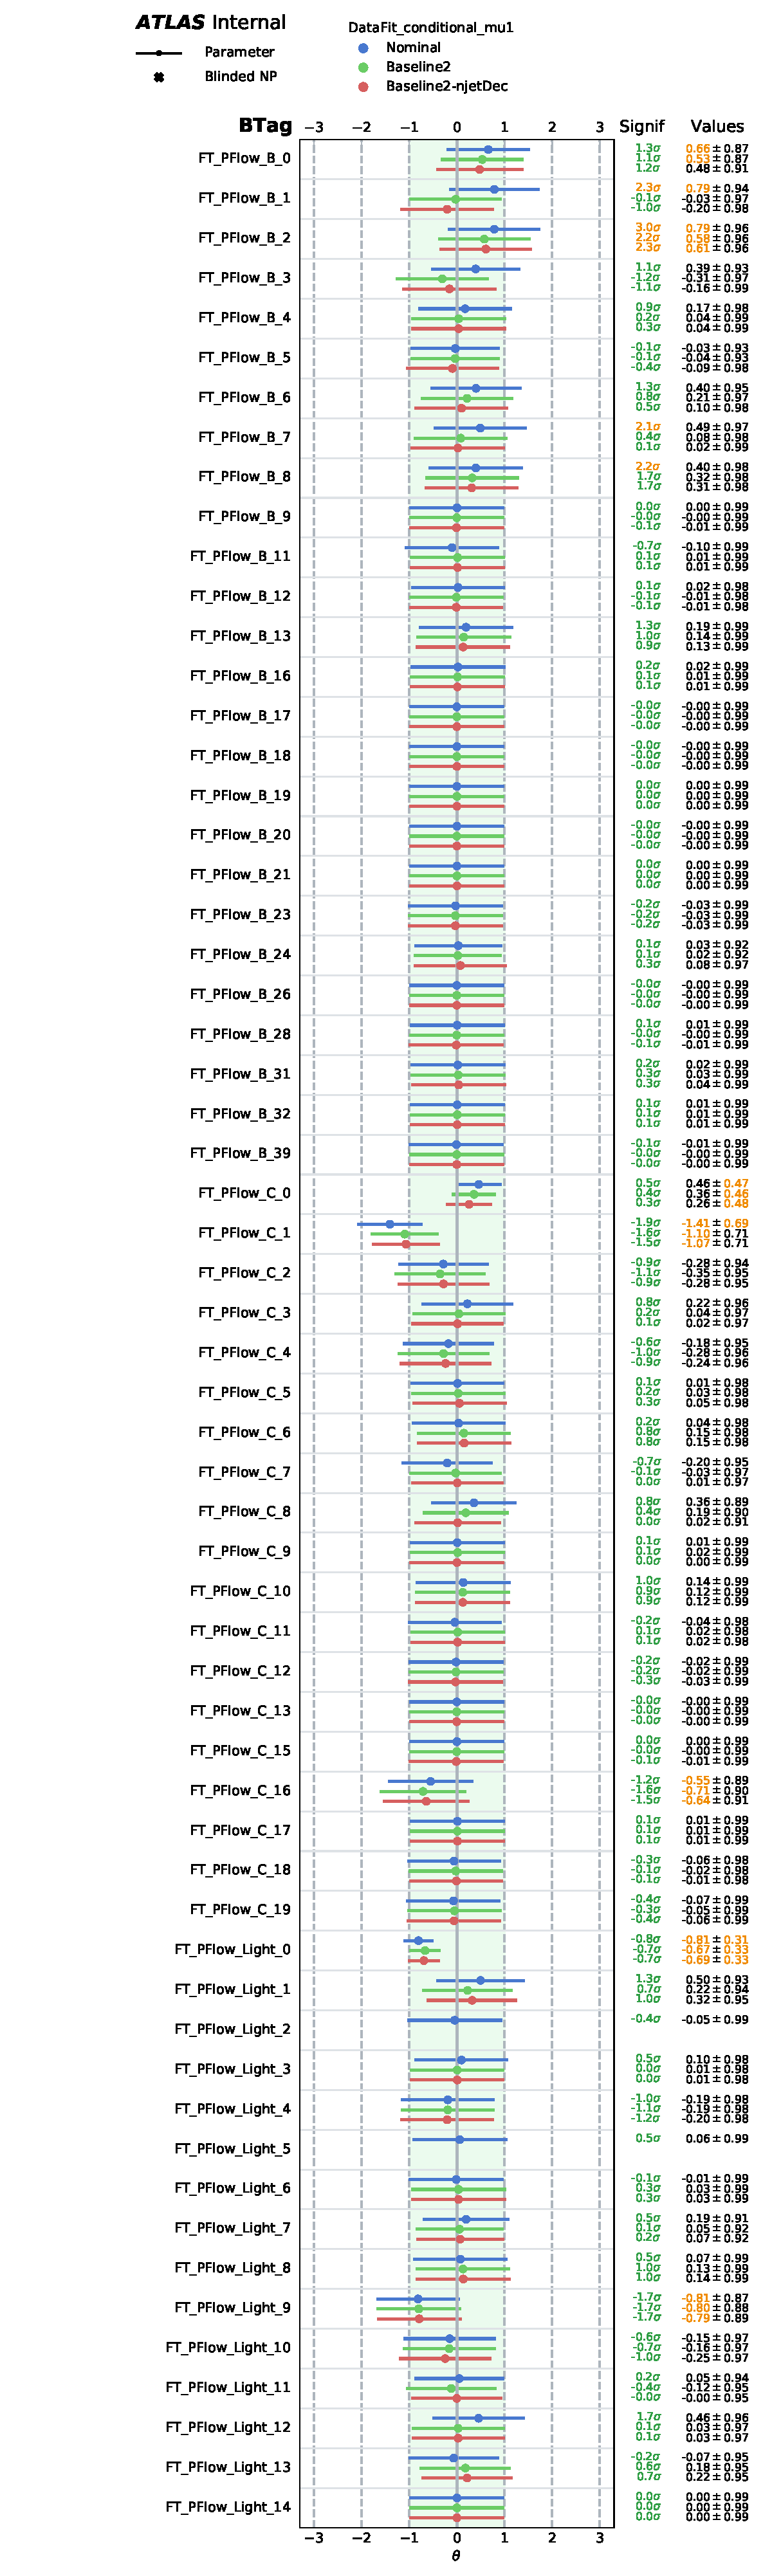
\includegraphics[scale=0.36]{Images/VH/clean_pull/NP_BTag.pdf}
\caption{Flavour tagging pulls.} 
\label{fig:pullsFTAG}
\end{subfigure}
\caption{Pulls for the 012L fit with the several baselines. Blue: nominal; green: baseline 2; red: baseline 2 + nJetDec.}
\label{fig:pulls}
\end{figure} 

The rest of Figure~\ref{fig:pullsTop} shows the most important top-related NPs. The METTrigTop, covering the differences between data and simulation in the MET trigger efficiency for top processes, is strongly pulled for all fit setups, something that requires further investigation from the analysis team. The NPs with name of the form \textit{NJetAcc\_Top*} list the nJet acceptances, a single one for the Nominal in blue and split in flavour for Baseline 2 in green. They are removed in Baseline 2 + nJetDec as in this case the NFs are floated separately for each number of jets region. This last setup is able to avoid incurring the rather large systematics induced by these 3-to-2 jets extrapolation uncertainties. Underneath the nJet acceptances, the pulls with names starting with \textit{Top\_mCC} represent shape systematics derived by considering the difference between the nominal samples and the alternative generators (such as Herwig and Powheg) or internal variations (like for the ISR). The $topCR\_extrap$ are the topCR-SR extrapolation uncertainties which are only applied in the Nominal setup. For the Baseline 2 variations, the flavour tagging NPs and associated pulls are able to cover this extrapolation with minimal changes to the Nominal, as shown in Figure~\ref{fig:pullsFTAG}. Through these different groups, the interesting observation is that the Baseline 2 + nJetDec performs similarly to the Baseline 2 and Nominal, despite having a much simpler structure without nJet acceptances nor topCR extrapolations. A closer look at other NPs, such as the b-tagging pulls, confirms there is a good agreement between the different alternatives and no over-constraining is observed. \\

The expected prefit 95\% confidence limits on the signal strength of $VH(H\rightarrow c\bar{c})$ of these conditional data fits are: 
\begin{itemize}
\item Nominal: $12.60^{+4.94}_{-3.52}$ × \gls{sm}
\item Baseline 2: $12.75^{+4.99}_{-3.56}$ × \gls{sm}
\item Baseline 2 + nJetDec: $12.71^{+4.98}_{-3.55}$ × \gls{sm}
\end{itemize}
These values are consistent between the different fits. Comparing the fit setups, Baseline 2 + nJetDec is preferred to serve as a new nominal thanks to its simplified fit structure, its lower number of NPs and normalisation factors, the ability to constrain the components in several number of jet regions, and the freedom to use the topCR BL region as a validation region rather than as a control region. The obtained limits are significantly improved compared to the previous ATLAS result of 26 × \gls{sm} (31 × \gls{sm}) \cite{Collaboration:2721696} and are competitive with the recent CMS results of an observed (expected) upper limit of 14 $\times$ \gls{sm} (7.6 $\times$ \gls{sm}) \cite{arXiv:2205.05550}. The analysis is however still not concluded and improvements are still being pursued by fine-tuning the event selection to avoid large uncertainties as much as possible, including new MC samples with lower MC statistical uncertainties, as well as revisiting the modelling uncertainties all while monitoring the fit behaviour and carrying out similar studies to the present one for other regions and backgrounds. 

\section{Conclusion}
The $VH(H\rightarrow b\bar{b}/c\bar{c})$ analysis of Run 2 provides an exciting avenue to improve the competitivity of the ATLAS measurement of the charm Yukawa coupling. While the analysis is still ongoing, the harmonisation of the $VH(H\rightarrow b\bar{b})$ and $VH(H\rightarrow c\bar{c})$, the refinement of the top control region, the introduction of MVA sas discriminating variables, and the many other modifications pursued in the Combined Analysis already indicate significant gains will be made on the previously published result. The analysis is planned to wrap up in the following months and will be described in detail in the final DPhil dissertation. 

\clearpage

